\chapter{Security Practices}\label{ch:security-practices}
AWS provides a variety of services and tools which can be configured to ensure a high level of security within the
cloud architecture used for the deployment.
Cyber security is a vital aspect of any online service as it is important to protect the resources hosted on AWS from
cyberattacks and to prevent the web app itself from being taken off the web~\parencite{cavelty2010cyber}.
It is critical that the best security practices are followed to ensure a high level of security.
This chapter will detail the security measures taken during the deployment of the AWS architecture.

When configuring EC2, a KeyPair was set up for logging into the instance.
This KeyPair is stored on a secure \mintinline{zsh}|.pem| file which should only be accessible to those who created
the EC2 instance.
The KeyPair is required to log into the instance and, therefore, only the authorised users who are part of the
development team have access to editing the EC2 instance.

\begin{figure}[!htbp]
    \centering
    \begin{minipage}{.5\textwidth}
        \centering
        \centering
        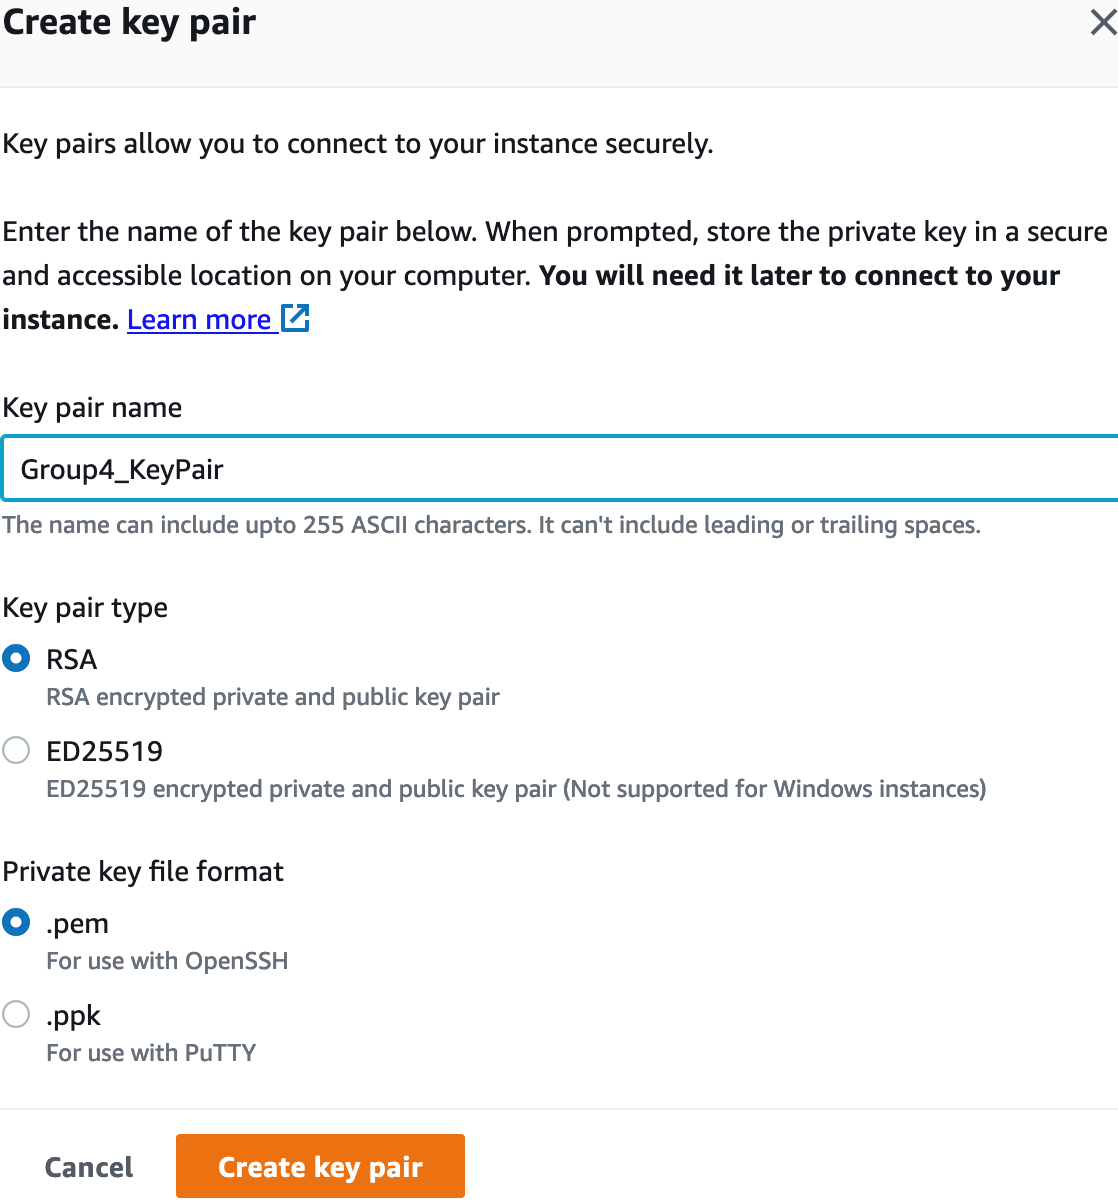
\includegraphics[width=1\linewidth]{resources/ec2/create-key-pair-2}
        \label{fig:create-keypair-pem}
    \end{minipage}%
    \begin{minipage}{.5\textwidth}
        \centering
        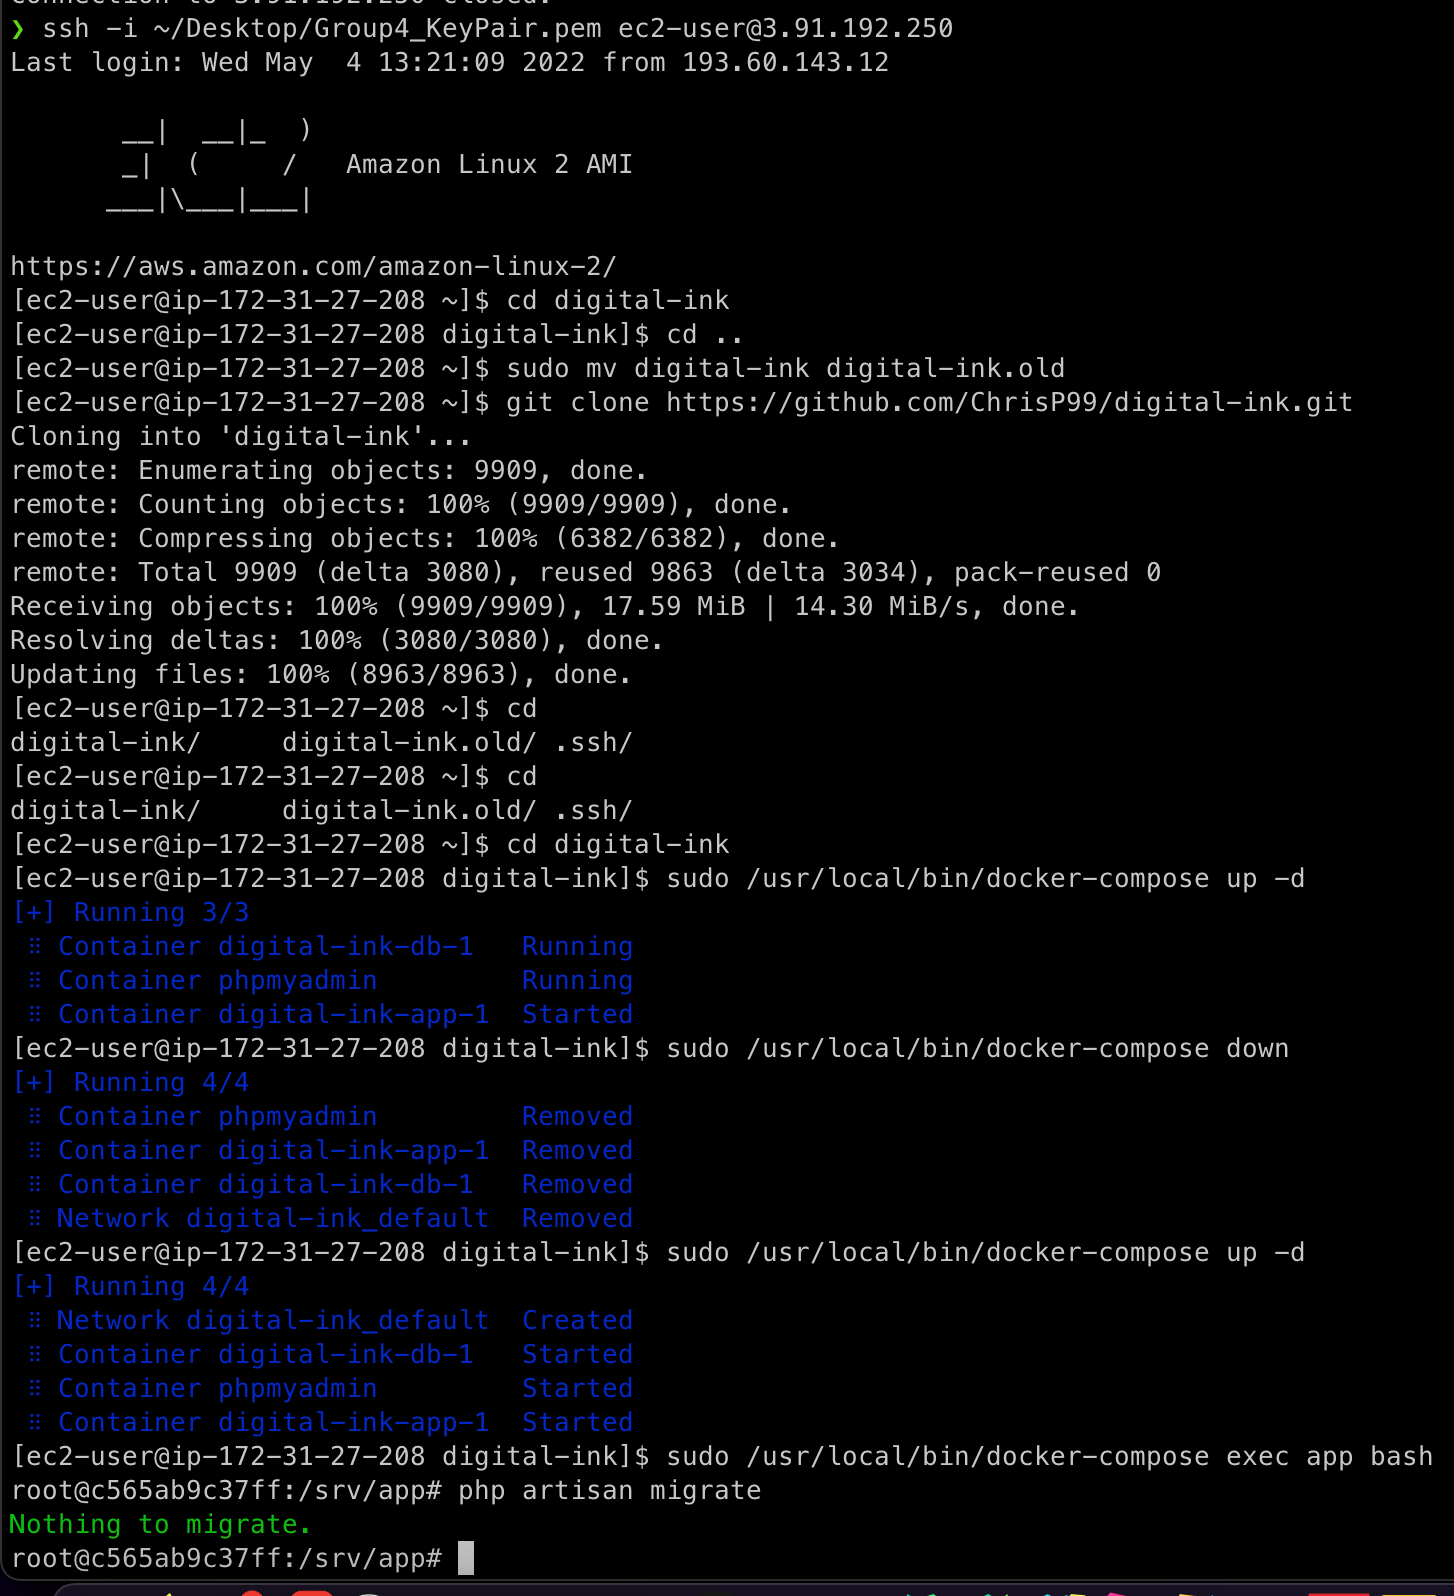
\includegraphics[width=1\linewidth]{resources/log-in-with-key-pair-2}
        \label{fig:log-in-keypair-pem}
    \end{minipage}
    \caption{Creating and using the KeyPair.}
    \label{fig:create-use-keypair}
\end{figure}

\clearpage
EC2 security groups are virtual firewalls used to control incoming and outgoing traffic for the AWS
deployment~\parencite{amazon2022amazon2}.
Security groups were implemented which limit connections to HTTP, HTTPS, SSH, and MySQL\@.
The HTTP, HTTPS, and MySQL connections were made accessible by public IP addresses as all users who access the web app
would require these permissions (HTTP and HTTPS to view the web app, and MySQL to query the database through the web
app).
The SSH connections are limited to one IP address (eduroam) as the public does not need access.
In a future deployment, the IP address with permission to access the SSH would be set to a private location, such as an
office, rather than eduroam.
During this deployment, the IP address of eduroam was allowed access due to the location in which the deployment was
configured.

\begin{figure}[!htbp]
    \centering
    \subfloat{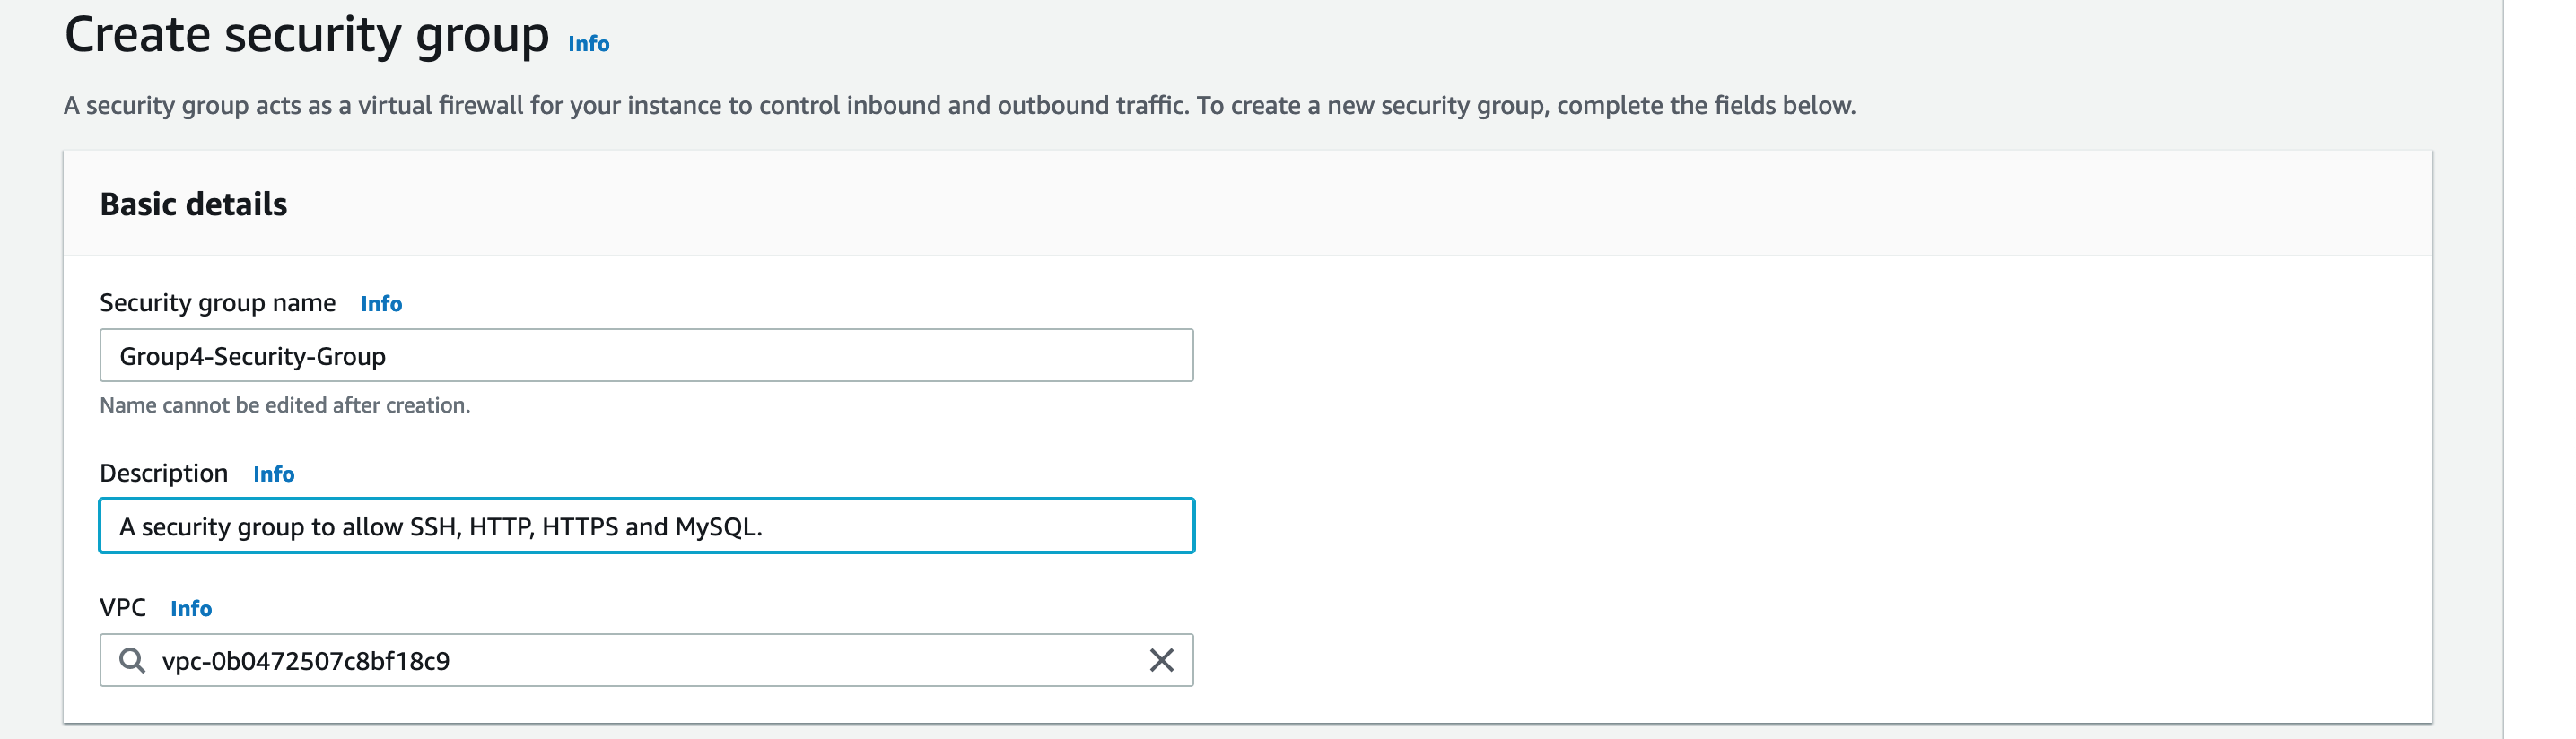
\includegraphics[width=125mm]{resources/security/security-group-name}}\hfill
    \subfloat{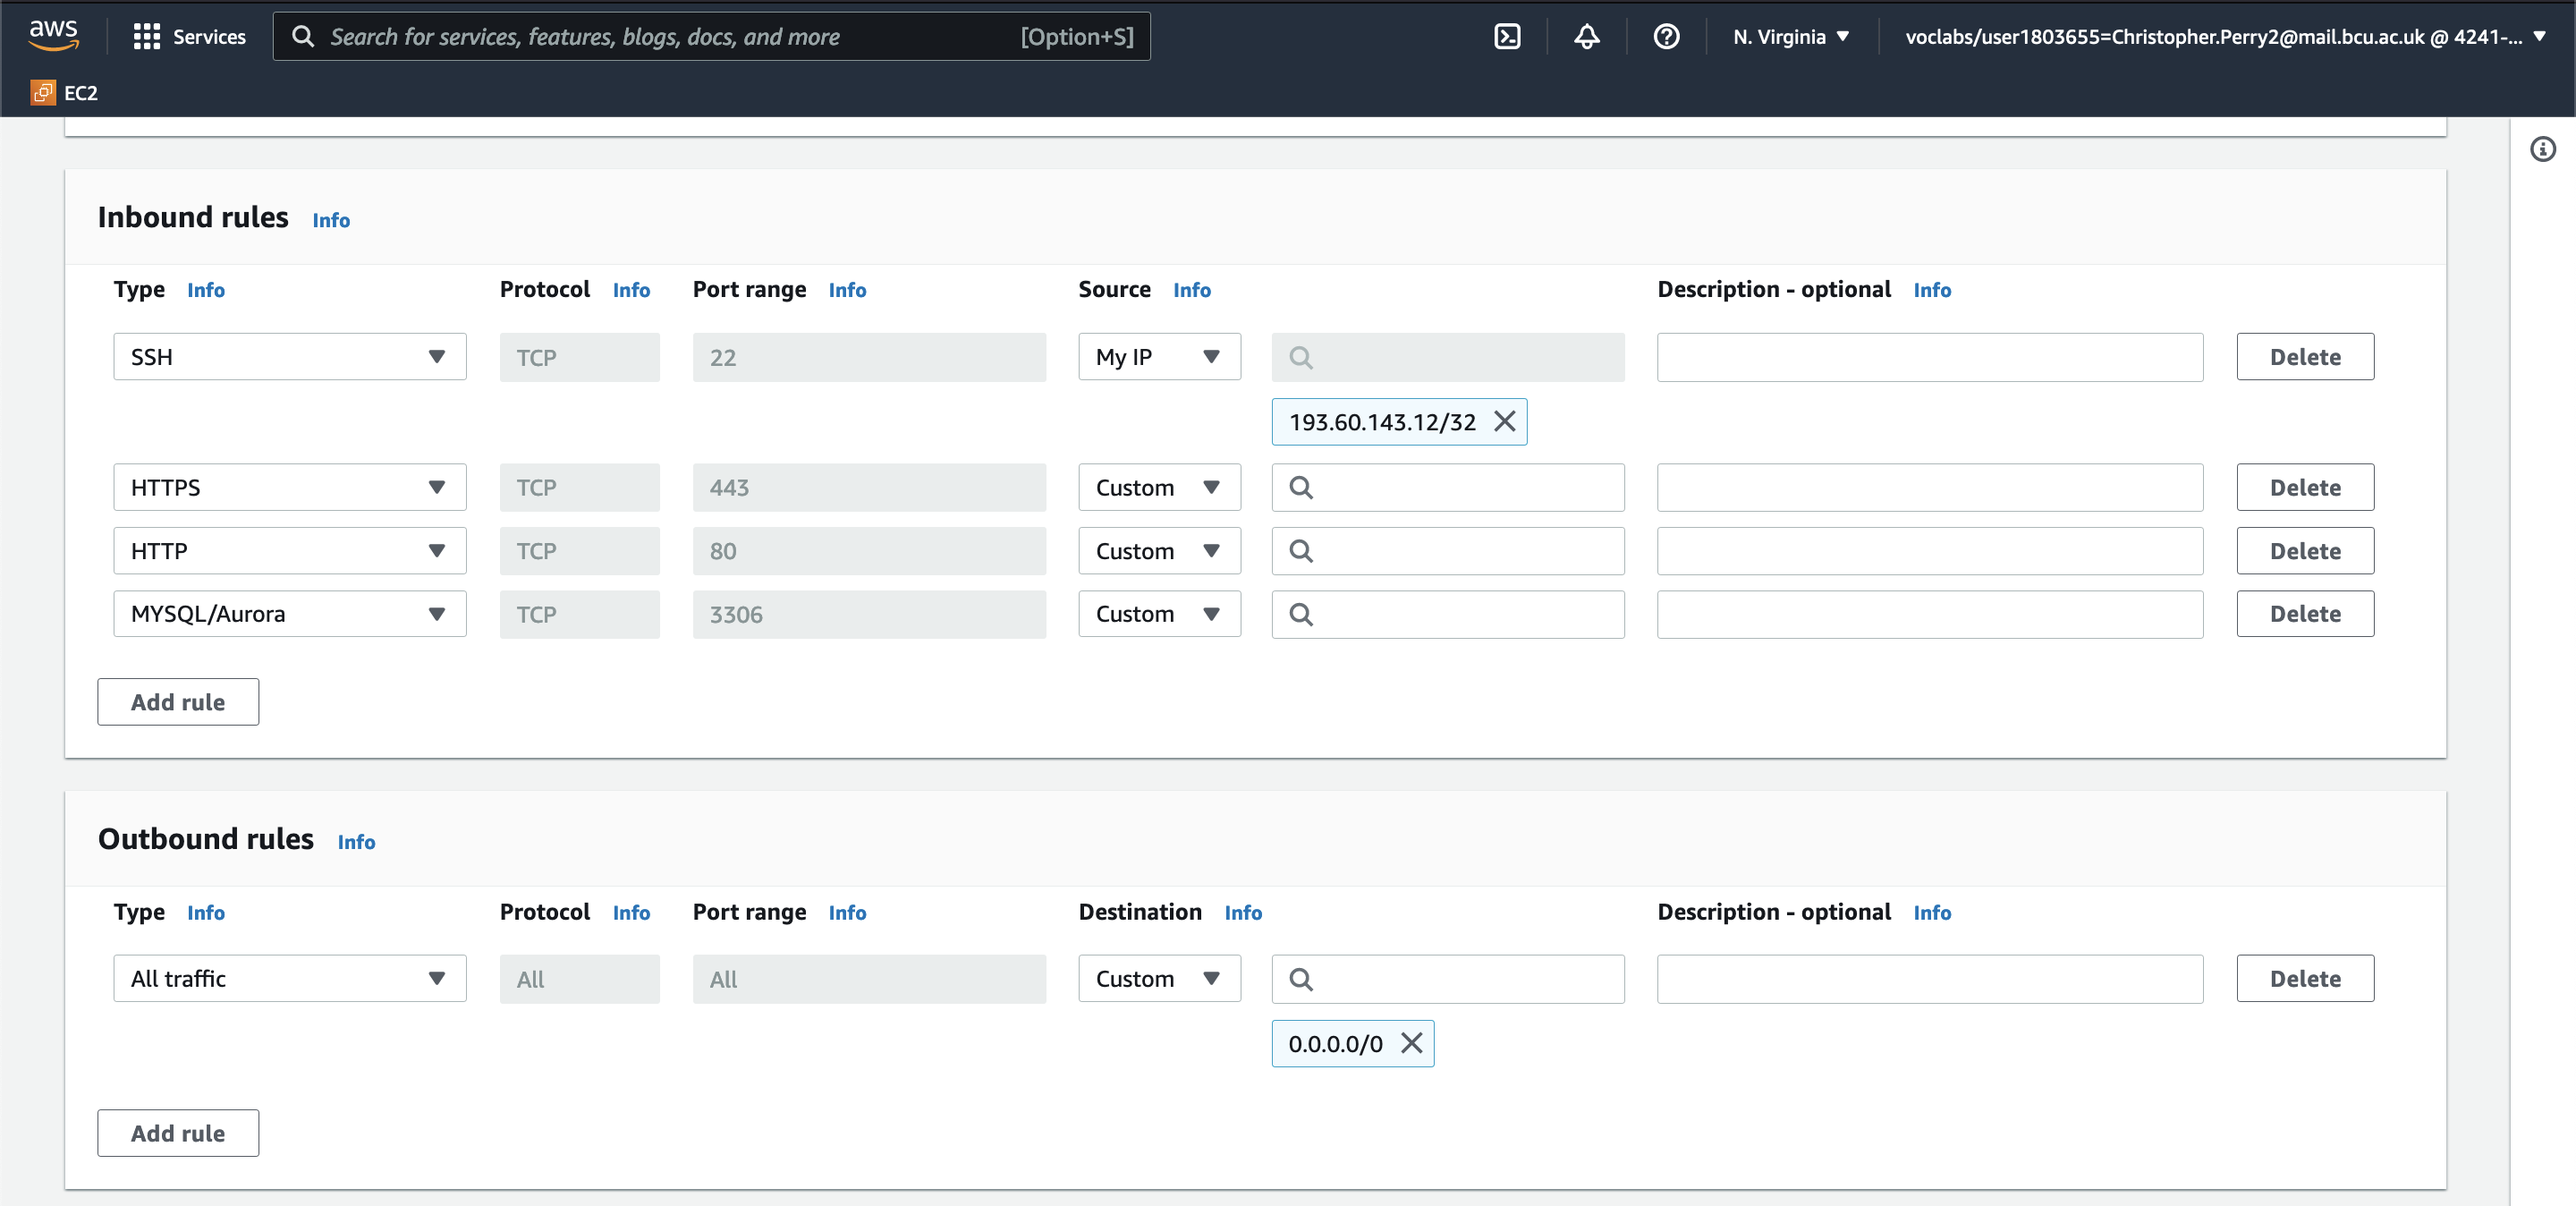
\includegraphics[width=125mm]{resources/security/security-group-rules}}\hfill
    \subfloat{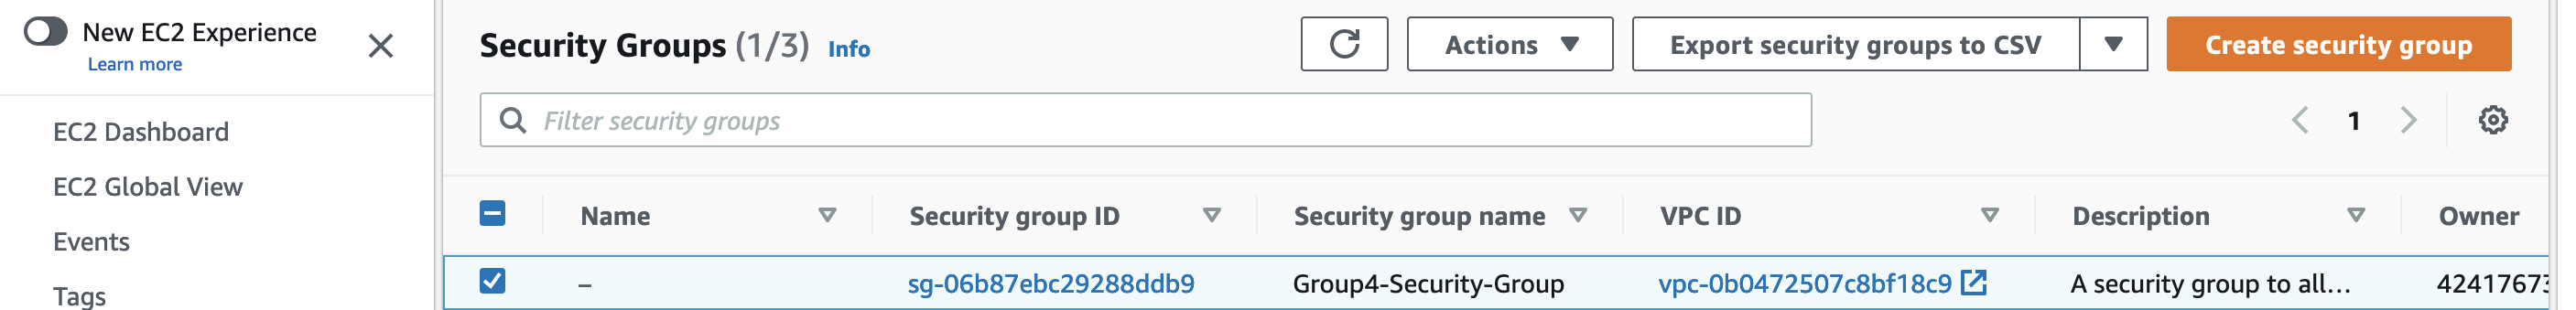
\includegraphics[width=125mm]{resources/security/security-group-created}}\hfill
    \subfloat{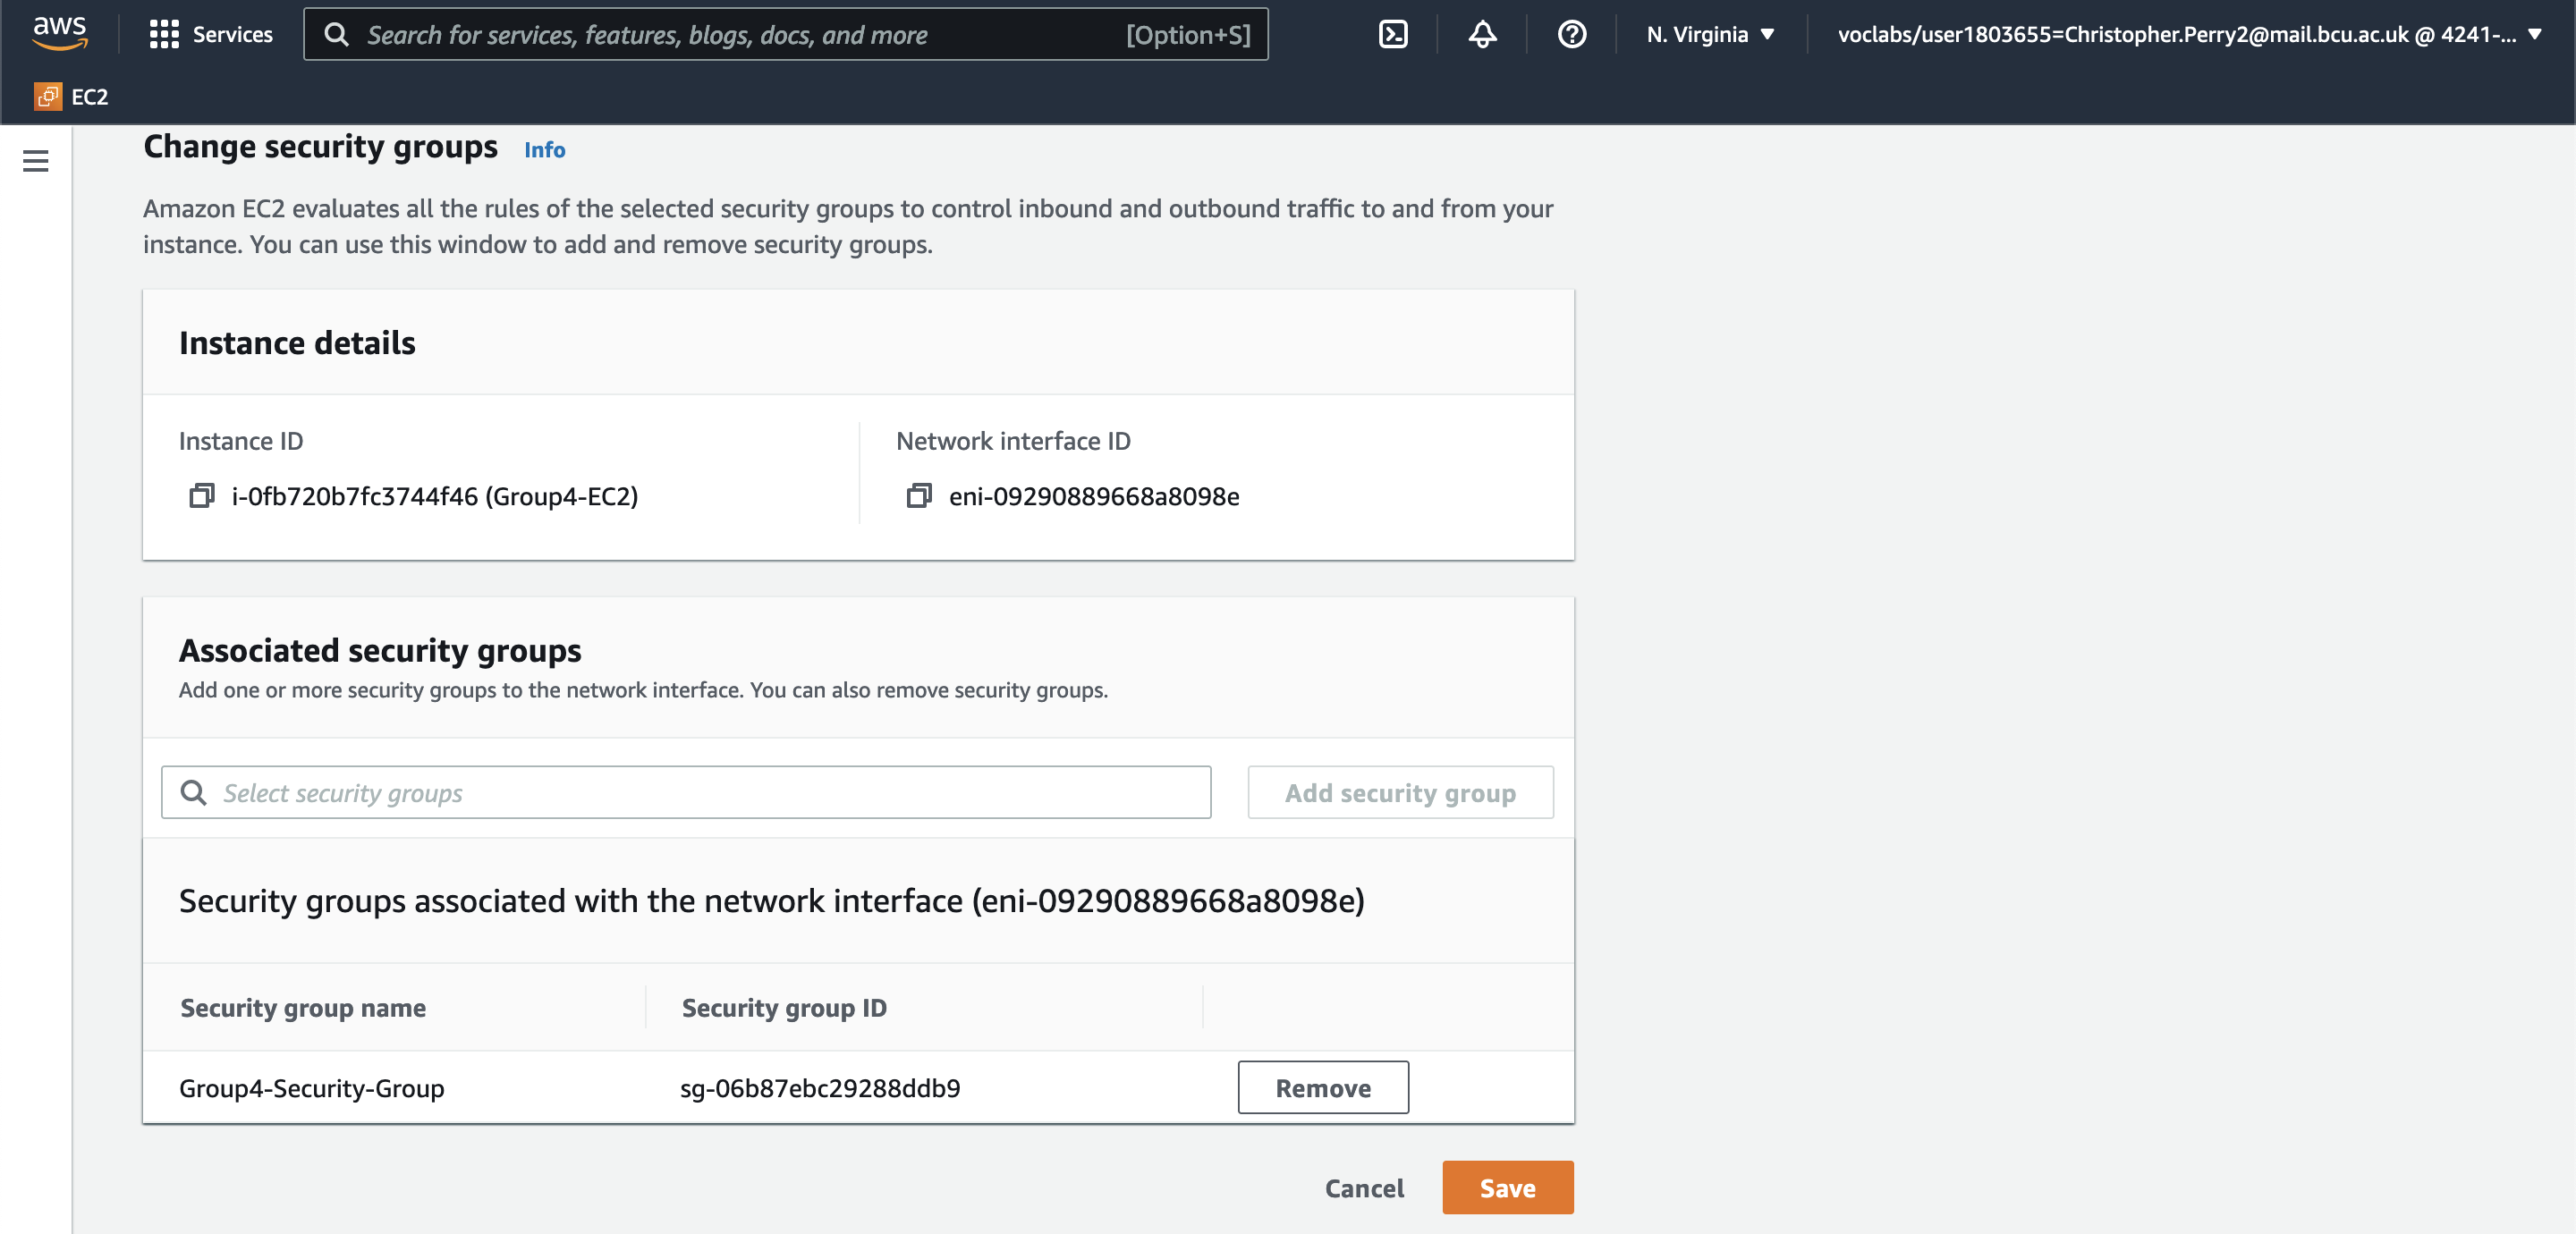
\includegraphics[width=125mm]{resources/security/security-group-associated}}
    \caption{Configuring security group.}
    \label{fig:security-groups}
\end{figure}

\clearpage
IAM is an AWS service which provides fine-tuned access control across the entire AWS deployment by creating a policy
which specifies which users have permission to access certain features and resources~\parencite{amazon2022aws2}.
Ideally, this would be implemented for security purposes.
Unfortunately, this feature could not be used due to restricted permissions.

\begin{figure}[!htbp]
    \centering
    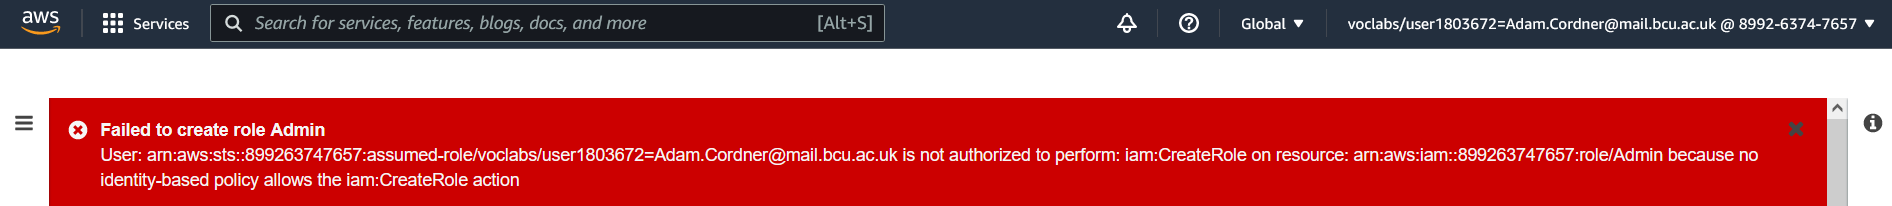
\includegraphics[width=\textwidth]{resources/iam-denied}
    \caption{Restricted permissions preventing the creation of IAM roles.}
    \label{fig:iam-denied-security}
\end{figure}

The S3 bucket was configured to use server-side encryption to safely store the data in the bucket.
This was done by specifying to use an Amazon S3-managed key (SSE-S3), i.e. an encryption key which Amazon S3
automatically creates, manages, and uses to encrypt the data.

\begin{figure}[!htbp]
    \centering
    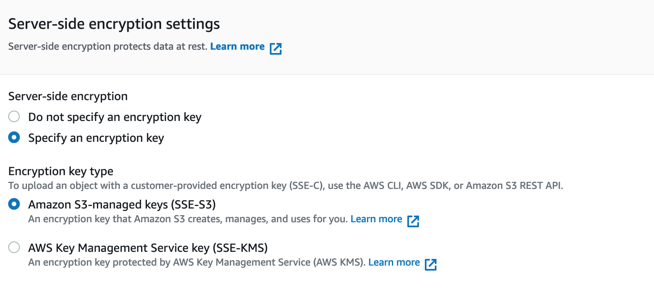
\includegraphics[width=\textwidth]{resources/s3/s3_encryption}
    \caption{S3 bucket encryption settings.}
    \label{fig:s3-encryption}
\end{figure}

\clearpage
When setting up the RDS for the web app, database authentication was configured to require password authentication.
This means that direct access to the SQL database requires the use of a master username and a master password generated
by AWS.

\begin{figure}[!htbp]
    \centering
    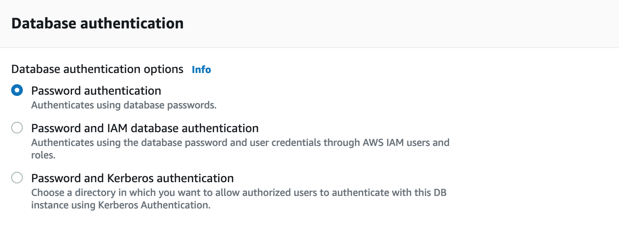
\includegraphics[width=\textwidth]{resources/rds_authentication}
    \caption{Setting up database authentication.}
    \label{fig:setup-rds-auth}
\end{figure}

\begin{figure}[!htbp]
    \centering
    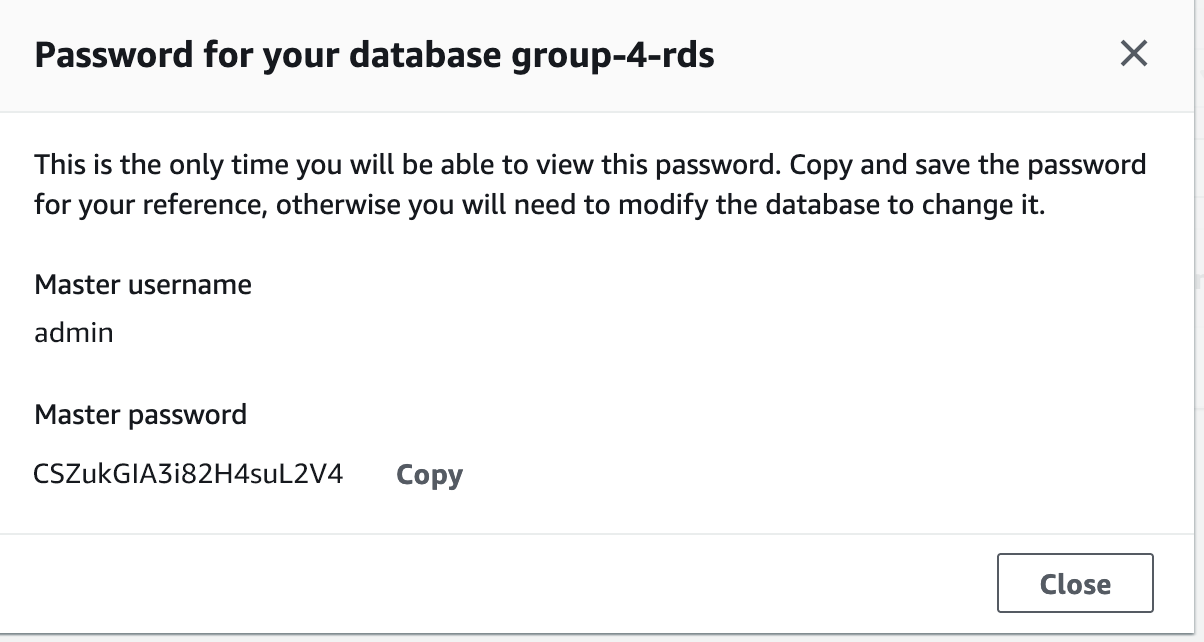
\includegraphics[width=\textwidth]{resources/RDS_password}
    \caption{Viewing log in details for database authentication.}
    \label{fig:view-rds-auth}
\end{figure}
